Se denominan algoritmos de \textit{clustering} aquellos algoritmos de aprendizaje no supervisado que agrupan los elementos de un conjunto de datos en conjuntos (clusters) de modo que los objetos pertenecientes a un mismo cluster sean más similares que aquellos en clusters distintos.
Su aplicación permite simplificar la estructura del conjunto de datos, convirtiéndolo en uno más pequeño y fácilmente manipulable;
o como en el caso que ocupa este trabajo, encontrar grupos de especial significación para el problema, como pueden ser agrupaciones de segmentos de audio correspondientes a vocalizaciones semejantes de individuos misma especie animal.

% Wikipedia
Los algoritmos de clustering difieren significativamente en su noción de qué constituye un cluster y cómo hallarlos eficientemente.
Algunas de las nociones de cluster más populares incluyen grupos con pequeñas distancias entre sus integrantes, áreas de alta densidad en el espacio de datos, o distribuciones estadísticas particulares.
El algoritmo más apropiado para un problema, así como su configuración de parámetros (incluyendo la función de distancia a emplear, el umbral de densidad o el número de clusters esperado) es altamente dependiente de las características del conjunto de datos y del uso que se desea dar a los resultados obtenidos.

La determinación del número de conjuntos es a menudo un problema en sí;
algunos algoritmos lo hayan como parte de su funcionamiento, mientras que otros requieren dicho valor como entrada.
Al proceso de decisión del algoritmo y la combinación de parámetros de mejor ajuste al problema, se le conoce como \textit{selección del modelo};
y las diferentes medidas para la evaluación de los resultados producidos por un modelo dado, con dicha finalidad, es un tema abordado más adelante en este trabajo.

En las siguientes secciones se explican los principales algoritmos de clustering que serán empleados en este trabajo.

\section{Clustering Particional}\label{sec:clusteringParticional}
A continuación es discutido el algoritmo de clustering conocido como K-Means, uno de los más simples y eficientes existentes en la literatura.
Luego de describir en detalle el algoritmo, se analizan algunos de los principales factores que influyen sobre sus resultados.
Finalmente, se presenta una variación de K-Means que busca disminuir la complejidad computacional del algoritmo.

\subsection{K-Means}\label{subsec:k-means}

K-Means~\cite{MacQueen67} es el algoritmo de clustering particional más empleado~\cite{Aggarawal13}.
Comienza seleccionando $K$ puntos representativos como \textit{centroides} iniciales, donde $K$ es un parámetro manualmente especificado por el usuario, siendo este el número deseado de clusters a obtener.
Cada punto del conjunto de datos es luego asignado al centroide más cercano basándose en una medida de proximidad determinada.
Una vez se han formado los clusters, los centroides para cada cluster son actualizados a un nuevo punto.
De manera iterativa, el algoritmo repite estos dos pasos hasta que los centroides no cambien o algún criterio de convergencia alternativo sea cumplido.
K-Means es un algoritmo \textit{greedy} con convergencia garantizada a un mínimo local~\cite{Selim84} pero, visto como un problema de optimización, ha sido demostrado que hallar el mínimo de su función objetivo es NP-Hard~\cite{Manning08}.
En la práctica, suele usarse como criterio de convergencia una versión relajada, continuándose las iteraciones hasta que menos del 1\% de los puntos cambien de cluster.

\begin{algorithm}
    \caption{K-Means}
    \label{algorithm:KMeans}
    Seleccionar $K$ puntos como centroides\;
    \Repeat{Se cumple criterio de convergencia}{
    Formar $K$ clusters asignando cada punto al centroide más próximo\;
    Recomputar el centroide de cada cluster\;
    }
\end{algorithm}

La elección de la medida de proximidad para calcular el centroide más cercano a cada punto puede afectar significativamente las asignaciones y la calidad de la solución final.
Medidas como la distancia Manhattan (norma $L_1$), la distancia euclidiana (norma $L_2$) y la similitud coseno son frecuentemente empleadas, especialmente la segunda.
Tanto la medida de proximidad como el valor de $K$ son determinantes en la configuración de clusters producida por K-Means.

Si se analiza este algoritmo como un problema de optimización, entonces estaría minimizándose la función objetivo de K-Means conocida como \textit{Suma de Errores Cuadráticos} (SSE por sus siglas en inglés), cuya formulación matemática se presenta a continuación.

Dado un conjunto de datos $D={x_1,x_2,\dots,x_N}$ de $N$ puntos, y denotado el conjunto de clusters obtenido tras aplicar K-Means como $C={C_1,C_2,\dots,C_k,\dots,C_K}$;
la SSE para $C$ es definida en la ecuación~(\ref{eq:SSE}) donde $c_k$ es el centroide del cluster $C_k$.

\begin{equation}
    \label{eq:SSE}
    SSE(C)=\sum_{k=1}^{K}{\sum_{x_{i}\in C_k}{dist(x_i, c_k)^2}}
\end{equation}

En otras palabras, se calcula el error de cada punto de los datos, es decir, su distancia al centroide más próximo, y luego es computada la suma de los cuadrados de dichos errores.
Dados dos conjuntos de clusters obtenidos aplicando dos diferentes corridas de K-Means, sería preferible conservar el de menor SSE puesto que esto significaría que los centroides hallados en esa corrida constituyen una mejor representación de los puntos en sus clusters.
De ahí que el resultado de minimizar la función SSE represente el conjunto de clusters óptimo.

Los centroides que minimizan la SSE son la media de los puntos de cada cluster~\cite{Tan05}.
El centroide del $k$-ésimo cluster, $c_k$, quedaría entonces definido según la ecuación~(\ref{eq:centroid}).

\begin{equation}
    \label{eq:centroid}
    c_{k}=\frac{1}{|C_k|}\sum_{x_{i}\in C_k}{x_i}
\end{equation}

Los pasos 3 y 4 del algoritmo~\ref{algorithm:KMeans} directamente intentan minimizar la SSE. El paso 3 forma clusters asignando los puntos al centroide más cercano, lo que minimiza la SSE de dicho conjunto de centroides.
Asimismo, el paso 4 recomputa los centroides, produciendo un nuevo conjunto de menor SSE, en correspondencia con la ecuación ~(\ref{eq:centroid}).
Sin embargo, como se mencionó anteriormente, estos pasos solamente garantizan la convergencia de K-Means a un mínimo local de la función SSE, puesto que la optimizan partiendo de una selección específica de centroides y cantidad de estos, en lugar de todas las posibles opciones.

\subsubsection{Selección de centroides iniciales}

En~\cite{MacQueen67} se propone un simple método de inicialización consistente en seleccionar los $K$ centroides de modo aleatorio.
Este es ampliamente usado en la literatura por su sencillez, aunque tiene la desventaja de que puede producir resultados muy diferentes en varias corridas del algoritmo, algunos de mayor calidad que otros.

Se han popularizado otras variantes de selección de los centroides, con el propósito de aumentar la efectividad y consistencia en los resultados de K-Means.
Uno de ellos es tomar una muestra de puntos y agruparlos empleando una técnica de clustering jerárquico.
Una vez formados $K$ clusters, se toman sus centroides y se inicializa K-Means con estos.
Este enfoque a menudo ofrece buenos resultados, pero solamente resulta práctico si la muestra tomada es relativamente pequeña (de un orden entre $10^2$ y $10^3$) y $K$ es relativamente pequeño comparado con el tamaño de dicha muestra~\cite{Tan05}.

Otra variante, conocida como \textbf{K-Means++}~\cite{Arthur07}, consiste en primeramente seleccionar un punto de manera aleatoria o tomando el centroide de todos los puntos.
Luego, se selecciona el punto más alejado de los centroides formados con anterioridad y se repite este paso hasta obtener $K$ centroides iniciales.

\subsubsection{Estimación del número de clusters}

K-Means es un algoritmo extremadamente dependiente del valor de $K$ seleccionado por el usuario.
La decisión de tal número constituye uno de los mayores desafíos, si no el mayor, al hacer uso de este algoritmo.
Es por esto que numerosos trabajos se han enfocado en el área de determinar el $K$ más apropiado, y varios métodos han sido desarrollados con tal propósito.
A continuación se mencionan algunos de los más generalizados.

\begin{enumerate}
    \item \textbf{Índice de Calinski-Harabasz}~\cite{Calinski74}: Está definido por la ecuación~(\ref{eq:CH}):
    \begin{equation}
        \label{eq:CH}
        CH(K)=\frac{\frac{B(K)}{K-1}}{\frac{W(K)}{N-K}}
    \end{equation}
    donde $N$ representa la cardinalidad del conjunto de datos.
    El número de clusters es seleccionado maximizando la función dada en la ecuación~(\ref{eq:CH}).
    $B(K)$ y $W(K)$ constituyen las sumas de los cuadrados de las distancias intra e inter-cluster respectivamente (dados $K$ clusters).

    \item \textbf{Estadística de Brecha}\footnote{\textit{Gap Statistic} en inglés.}~\cite{Tibshirani01}: En este método se generan $B$ conjuntos de datos que siguen una distribución uniforme en el mismo intervalo que los valores del original.
    Sea $W_{b}^{*}(K)$ la suma de los cuadrados de las distancias intra-cluster del $b$-ésimo conjunto de datos, se plantea entonces la siguiente ecuación:
    \begin{equation}
        Gap(K) = \frac{1}{B} \times\sum_{b}{\log(W_{b}^{*}(K)) - \log(W(K))}
    \end{equation}
    El número de clusters seleccionado es el menor valor de $K$ que satisfaga la ecuación~(\ref{eq:Gap}):
    \begin{equation}
        \label{eq:Gap}
        Gap(K) \geq Gap(K+1) - S_{k+1}
    \end{equation}
    donde $S_{k+1}$ es el valor de la desviación estándar de $\log(W_{b}^{*}(K+1))$.

    \item \textbf{Criterio de Información de Akaike (AIC)}~\cite{Yeung01}: Sea $M$ el número de dimensiones del conjunto de datos, $K$ se calcula a partir de la ecuación~(\ref{eq:AIC}).
    \begin{equation}
        \label{eq:AIC}
        K=argmin_{K}[SSE(K)+2M K]
    \end{equation}

    \item \textbf{Coeficiente de Silueta}\footnote{\textit{Silhouette Coefficient} en inglés.}~\cite{Kaufman90}: Su formulación considera tanto la distancia intra-cluster como la inter-cluster.
    Para un punto dado $x_i$, primero se calcula el promedio de las distancias de este a todos los puntos del mismo cluster ($a_i$).
    Luego por cada cluster que no contiene a $x_i$, se computa el promedio de las distancias de $x_i$ a sus integrantes ($b_i$).
    Usando estos dos valores, se estima el coeficiente de silueta de un punto como el cociente entre su diferencia y el mayor de ambos.
    El promedio de todos los coeficientes en el conjunto de datos puede ser empleado para evaluar la calidad de un clustering.
    Mayores valores se corresponden con modelos cuyos clusters se encuentran mejor definidos.
    \begin{equation}
        S = \frac{\sum_{i=1}^{N}{\frac{b_{i}-a_{i}}{\max(a_i,b_i)}}}{N}
    \end{equation}
\end{enumerate}

\subsubsection{Complejidad espacial y temporal}

Los requerimientos de espacio de memoria para K-Means son relativamente pequeños puesto que solamente los puntos y los centroides son almacenados por el algoritmo.
Específicamente, la cantidad de memoria empleada es $O((n+K)m)$, donde $n$ es el número de puntos y $m$ la cantidad de atributos (dimensionalidad) de estos.
Los requisitos de tiempo de este algoritmo son igualmente bajos, es básicamente lineal respecto al tamaño del conjunto de datos.
En particular, el tiempo requerido es $O(I \cdot K \cdot m \cdot n)$, donde $I$ es el número de iteraciones necesarias para converger.
A menudo $I$ es suficientemente pequeño, y usualmente puede ser considerado como un valor constante y despreciable.
De esta forma, K-Means es lineal respecto al tamaño del conjunto de datos $n$, y es muy eficiente siempre que el número de clusters $K$ sea significativamente menor que $n$~\cite{Tan05}.

\subsection{Mini-batch K-Means}\label{subsec:miniBatchKMeans}

Mini-batch K-Means es una variante del algoritmo K-Means que emplea \textit{mini-batches} con el fin de reducir el tiempo de computación, sin afectar la función objetivo a optimizar.
Los \textit{mini-batches} son subconjuntos del conjunto de datos sobre el que se aplica el algoritmo, tomados mediante un muestreo aleatorio en cada iteración.
Estos reducen drásticamente la cantidad de cómputo necesario para converger a un óptimo local.

\begin{algorithm}
    \caption{Mini-batch K-Means}
    \label{algorithm:MiniBatchKMeans}
    Seleccionar $K$ puntos como centroides\;
    \Repeat{Se cumple criterio de convergencia}{
    Tomar una muestra aleatoria de $b$ puntos del conjunto de datos\;
    Asignar cada punto de la muestra al cluster que corresponda al centroide más próximo\;
    Recomputar el centroide de cada cluster\;
    }
\end{algorithm}

Al recomputar los centroides durante cada iteración se tienen en cuenta tanto los puntos de la muestra recién asignados como los asignados durante las iteraciones anteriores.

El algoritmo Mini-batch K-Means converge a mayor velocidad que K-Means, aunque la calidad de sus resultados es menor.
No obstante, para aplicaciones prácticas, esta diferencia en calidad suele ser poco significativa~\cite{Sculley10}.

\section{Clustering Jerárquico Aglomerativo}\label{sec:clusteringJerárquicoAglomerativo}
Las técnicas de clustering jerárquico son, como las de clustering particional, relativamente antiguas en comparación con muchas otras que analizaremos más adelante.
Aún así se mantienen entre las más usadas en la actualidad.
Fueron desarrolladas con la finalidad de resolver algunas de las desventajas de los algoritmos de clustering particional que hemos visto, como su necesidad de una cantidad de clusters prefijada y su naturaleza no determinista.


\section{Clustering Basado en Densidad}\label{sec:Dbscan}
Algoritmos como K-Means presentan dificultades para identificar clusters cuando las distancias entre elementos de un mismo conjunto es mayor que la de elementos de conjuntos distintos.
En estos casos, puesto que K-Means busca minimizar la distancia entre los elementos dentro de un mismo cluster, producirá clusters que difieran significativamente de los grupos <<correctos>>.
Podemos observar un ejemplo en el escenario de la figura~\ref{img:kmeans-dbscan}, donde se compara el resultado de K-Means con el del algoritmo que analizamos en esta sección, conocido como \textit{DBSCAN}.

\begin{figure}[!h]
    \centering
    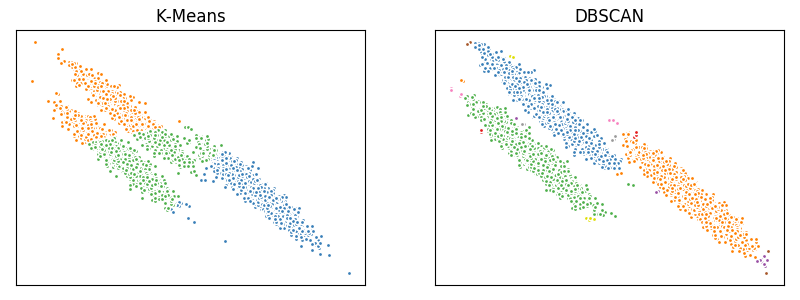
\includegraphics[width=\textwidth]{kmeans-dbscan.png}
    \caption{Resultados de los algoritmos K-Means y DBSCAN ejecutados sobre un conjunto de datos que sigue una distribución anisotrópica.}
    \label{img:kmeans-dbscan}
\end{figure}

En la imagen podemos observar asimismo el comportamiento de otro algoritmo sobre el mismo conjunto de datos.
En esta sección abordamos el algoritmo en cuestión, denominado \textit{DBSCAN}~\footnote{Siglas en inglés de \textit{Density-based spatial clustering of applications with noise}.}, que forma parte del conjunto de algoritmos de clustering basados en la densidad de los datos.

Un cluster basado en el criterio de densidad de los puntos consiste en un área densa de puntos conectados, separado de otros clusters por áreas de menor densidad.

\subsection{Densidad}\label{subsec:densidad}

El algoritmo DBSCAN define la densidad alrededor de un punto como la cantidad de puntos localizados alrededor de este en un radio, $Eps$, específico.
El propio punto es incluido en este conteo.
En la figura~\ref{img:dbscan} se puede observar gráficamente esta definición.
En este caso número de puntos alrededor de $A$ es 7.

El valor del radio es determinante en la densidad de un punto.
Si este valor es suficientemente grande, entonces todos los puntos tendrán una densidad de $n$, el número de puntos en el conjunto de datos.
En cambio, si el radio es demasiado pequeño, la densidad de todos los puntos será igual a 1.
Más adelante discutiremos algunas estrategias para la selección de valores apropiados para el radio.

\begin{figure}[!h]
    \centering
    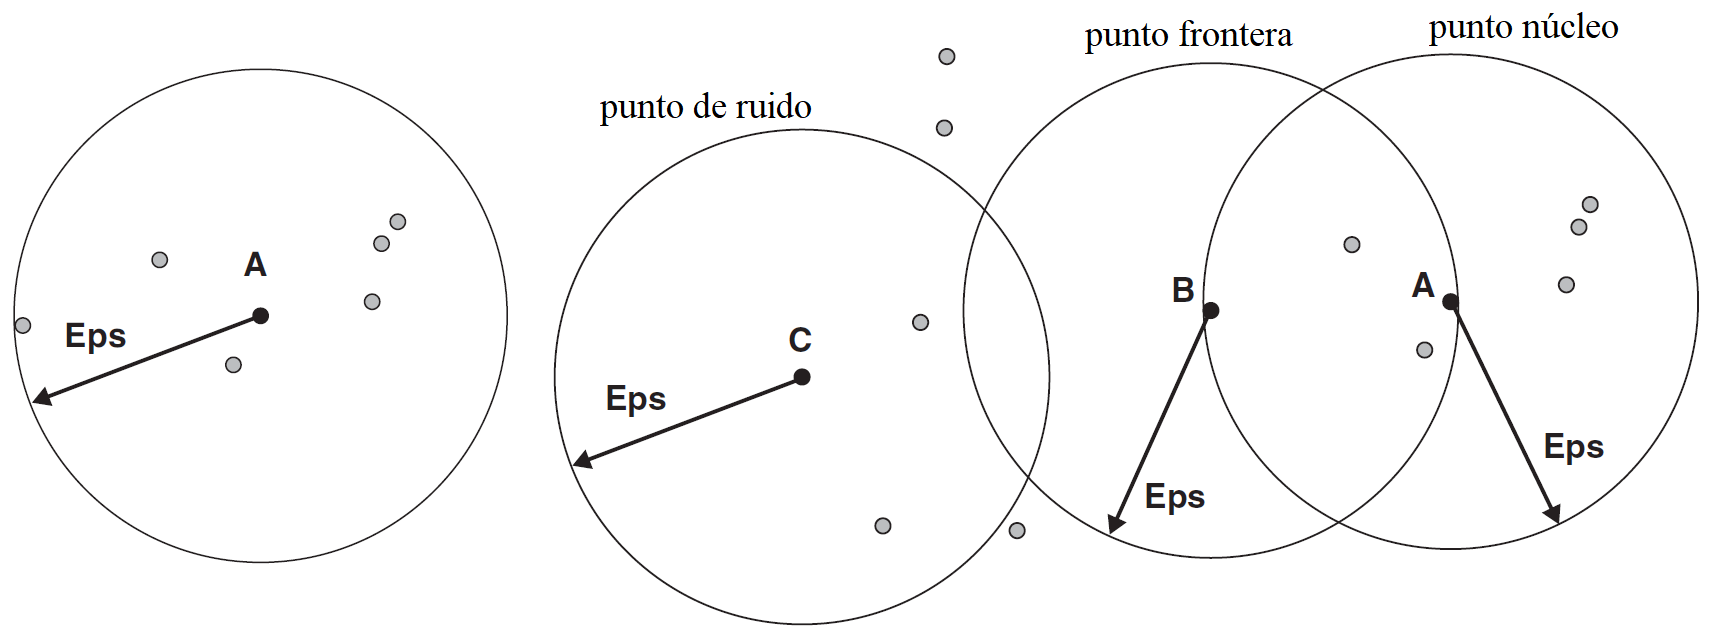
\includegraphics[width=\textwidth]{dbscan.png}
    \caption{Densidad en el entorno de un punto y clasificaciones de los puntos según su densidad. (Tomado de~\cite{Tan05}.)}
    \label{img:dbscan}
\end{figure}

De acuerdo con la densidad de un punto, estos pueden ser clasificados de la siguiente forma:

\begin{itemize}
    \item \textbf{Puntos núcleo}: Constituyen puntos de la región interna de un cluster basado en densidad.
    Un punto es núcleo si el número de puntos alrededor de este (incluyéndolo) supera o iguala un valor $MinPts$, especificado por el usuario.
    En la figura~\ref{img:dbscan} los puntos identificados con la letra $A$ son núcleos para el radio $Eps$ indicado si $MinPts\leq 7$.
    \item \textbf{Puntos frontera}: Un punto frontera es aquel que no cumple el criterio de núcleo, pero que forma parte de la vecindad de al menos uno de estos.
    En la figura~\ref{img:dbscan} $B$ es un punto frontera.
    \item \textbf{Puntos de ruido}: Un punto es de ruido si no es núcleo o frontera.
    En la figura~\ref{img:dbscan} $C$ es un punto de ruido.
\end{itemize}

\subsection{Algoritmo DBSCAN}\label{subsec:algoritmoDbscan}

A partir de las definiciones dadas de puntos núcleos, fronteras y de ruido, podemos describir el algoritmo DBSCAN del siguiente modo: Todo par de puntos núcleos cuya distancia sea no mayor que $Eps$ son asignados al mismo cluster.
De igual forma, los puntos fronteras son asignados al cluster de los puntos núcleos cuya distancia a estos sea menor o igual que $Eps$.
(En caso de estar en la vecindad de núcleos pertenecientes a clusters diferentes, un criterio específico debe ser determinado al programar el algoritmo).
Los puntos de ruido son descartados y no asignados a ningún cluster.

\begin{algorithm}
    \caption{DBSCAN}
    \label{algorithm:DBSCAN}
    Etiquetar todos los puntos como núcleo, frontera o ruido\;
    Eliminar los puntos de ruido\;
    Añadir una arista entre todo par de puntos núcleos que se encuentren a una distancia menor o igual que $Eps$\;
    Convertir cada componente conexa del grafo resultante en un cluster\;
    Asignar cada punto frontera a uno de los clusters de los puntos núcleos asociados a este\;
\end{algorithm}

\subsubsection{Complejidad espacial y temporal}

El algoritmo DBSCAN demora en ejecución un tiempo $O(n \cdot$ tiempo para encontrar puntos en una $Eps$-vecindad), donde $n$ es el número de puntos en el conjunto de datos.
En el peor caso, esta complejidad sería $O(n^2)$.
Sin embargo, el uso de determinadas estructuras de datos en espacios de pocas dimensiones, permite la recuperación eficiente de todos los puntos en un intervalo dado alrededor de un punto específico~\cite{Tan05};
en estos escenarios la complejidad puede llegar a ser $O(n\log n)$.
Los requerimientos de memoria de DBSCAN, aun en espacios de grandes dimensiones, son $O(n)$, puesto que solo es necesario mantener poca información relativa a cada punto, como puede ser el cluster al que pertenece, la clasificación, etc.
No obstante, este uso de memoria depende igualmente del comportamiento de la estructura de datos empleada para computar las vecindades.

\subsubsection{Selección de parámetros para DBSCAN}

Un criterio para determinar los parámetros es mediante la observación del comportamiento de la distancia de los puntos a su $k$-ésimo vecino más cercano, conocida como $k$-distancia.
Si un punto pertenece a un cluster, entonces su $k$-distancia debe ser un valor relativamente pequeño, siempre que $k$ no sea mayor que el tamaño del cluster.
Siempre que las densidades de los clusters no difieran radicalmente, en promedio, los valores de la $k$-distancias para puntos que pertenezcan a algún cluster no mostrarán un rango de valores muy amplio.
En cambio, para puntos que no pertenezcan a ningún cluster, es decir, de ruido, este valor sí estará situado muy por encima del rango antes mencionado.
De esta forma, si tomamos todos los puntos de un conjunto de datos, los ordenamos por su $k$-distancia y estas las representamos en una gráfica, deberíamos obtener una imagen donde existirá un punto de inflexión que se corresponda con el valor de la $k$-distancia a partir del cual los puntos se encuentran fuera de algún cluster.
Podemos entonces tomar dicho valor como el $Eps$ adecuado para el problema en cuestión.
En cuanto al valor de $MinPts$, este sería precisamente el $k$ seleccionado para calcular las distancias, pues los puntos cuya $k$-distancia sea menor que $Eps$ serán etiquetados como núcleos, mientras los demás serán fronteras o ruido.

% TODO Consider putting an example of graphic here

Es importante notar que el valor de $Eps$ resultante de este proceso dependerá del $k$ seleccionado al inicio.
Si $k$ es demasiado pequeño, algunos puntos de ruido situados muy próximos entre sí pudieran ser etiquetados incorrectamente como clusters.
Por otra parte, si $k$ es demasiado grandes, aquellos clusters cuya cantidad de elementos sea menor que $k$ no serán identificados correctamente.

Un defecto del algoritmo DBSCAN es que requiere que las densidades de los clusters (y del espacio de datos en general) muestren comportamientos semejantes.
Un ejemplo de esta afirmación podemos observarlo en la figura~\ref{img:density-issues}.
El ruido alrededor de los clusters $A$ y $B$ presenta la misma densidad que los clusters $C$ y $D$.
Si seleccionamos un $Eps$ suficientemente bajo para detectar a $C$ y $D$, sucederá entonces que $A$, $B$ y el ruido a su alrededor constituirán un mismo cluster.
En cambio si el $Eps$ es tan alto como para distinguir a $A$ y $B$ como clusters independientes, entonces los puntos que forman parte de $C$ y $D$ serán considerados ruido.

\begin{figure}[!h]
    \centering
    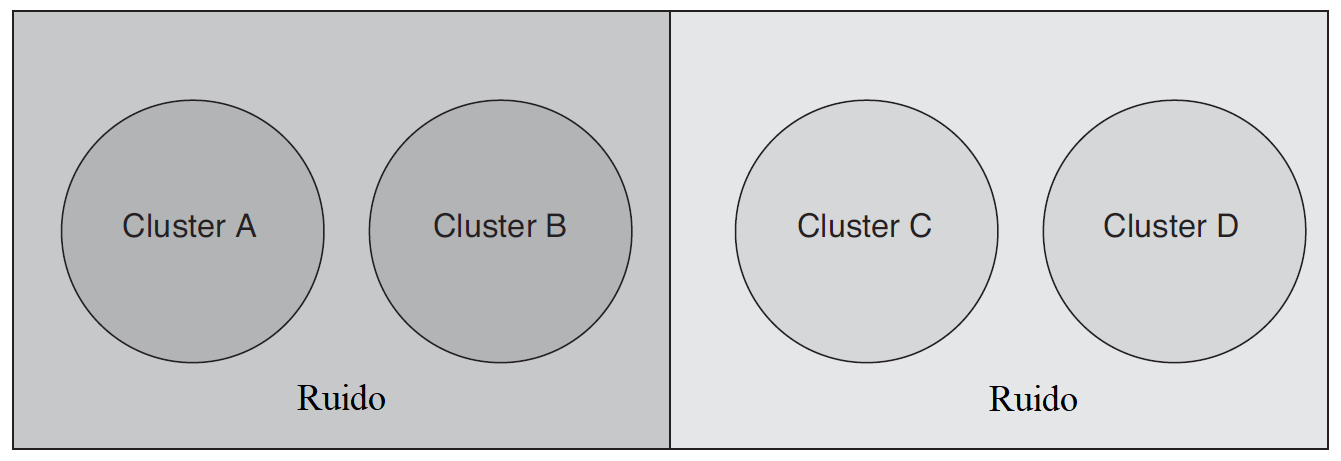
\includegraphics[width=\textwidth]{density-issues.png}
    \caption{Cuatro clusters en un entorno de ruido.
    Los tonos de gris más oscuros indican mayores densidades. (Tomado de~\cite{Tan05}.)}
    \label{img:density-issues}
\end{figure}

% TODO Consider adding HDBSCAN

\section{Clustering Basado en Probabilidades}\label{sec:clusteringBasadoEnProbabilidades}
Los algoritmos de clustering probabilísticos modelan el conjunto de datos a partir de la asunción de que este es generado mediante la combinación de determinadas distribuciones de probabilidad.
Estos algoritmos transforman el problema de clustering en el de estimar los parámetros para $K$ distribuciones de probabilidad.
Luego los puntos del conjunto de datos que se correspondan con una misma distribución se asociarán al mismo cluster.

En esta sección se analiza un modelo de clustering probabilístico ampliamente estudiado, conocido como \textit{Gaussian Mixture Model} (GMM);
así como la técnica \textit{Expectation-maximization}, empleada para estimarlo computacionalmente.

\subsection{Combinación de modelos}\label{subsec:mixtureModels}

Sea $X={x_1,\dots,x_N}$ un conjunto de datos de $N$ observaciones de una variable aleatoria $x$ con $D$ dimensiones.
Se asume que la variable $x_i$ sigue una distribución consistente con la combinación de $K$ \textbf{distribuciones componentes} (clusters), cada una instancia de una distribución para determinados parámetros.
Puede definirse entonces la función de densidad de $x_i$ como:

\begin{equation}
    \label{eq:mixtureModels}
    p(x_i)=\sum_{k=1}^{K}{\pi_k p(x_i|\theta_k)}
\end{equation}

\noindent
donde cada $\theta_k$ es el conjunto de parámetros específicos de la $k$-ésima componente y $p(x_i|\theta_k)$ su función de densidad.
Los pesos $\pi_k$, también conocidos como \textit{mixing probabilities}, deben satisfacer las condiciones $0\leq \pi_k \leq 1$ y $\sum_{k=1}^{K}{\pi_k}=1$.

Si bien la definición no establece ninguna restricción en cuanto al tipo de distribución que debe seguir cada componente;
en la práctica, para simplificar el estudio de estos modelos, suele asociarse una misma distribución a todas las componentes, variando únicamente sus parámetros.

\subsection{Gaussian Mixture Model}\label{subsec:GMM}

El modelo de clustering probabilístico más extendido es el de combinación de distribuciones normales, conocido en la literatura como \textit{Gaussian Mixture Model} (GMM)~\cite{Murphy12}.
Es asimismo, uno de los modelos de mayor uso en aplicaciones relacionadas con el análisis acústico~\cite{Kakar13,Kwan06,Lee08,Somervuo06,Virtanen18}.

La distribución normal, en el caso de una variable unidimensional $x$, tiene una función de densidad de la forma:

\begin{equation}
    \label{eq:singleGaussian}
    \mathcal{N}(x|\mu,\sigma^2)=\frac{1}{(2\pi\sigma^2)^{1/2}}\exp{(-\frac{1}{2\sigma^2}((x-\mu)^2)}
\end{equation}

\noindent
donde $\mu$ es la media y $\sigma^2$ la varianza.
Para el caso de $D$ dimensiones, la función toma la forma:

\begin{equation}
    \label{eq:multidimGaussian}
    \mathcal{N}(x|\mu,\Sigma)=\frac{1}{(2\pi)^{D/2}|\Sigma|^{1/2}}\exp{(-\frac{1}{2}(x-\mu)^T \Sigma^{-1}(x-\mu))}
\end{equation}

\noindent
donde $\mu$ es el vector $D$-dimensional de medias y $\Sigma$, de dimensión $D\times D$, la matriz de covarianza con determinante $|\Sigma|$.

En GMM cada componente corresponde a una distribución normal con determinados valores asociados a sus parámetros $\mu$ y $\Sigma$.
A partir de la ecuación~(\ref{eq:mixtureModels}) se puede entonces formular este modelo como:

\begin{equation}
    \label{eq:GMM}
    p(x_i|\Theta) = p(x_i|\pi,\mu,\Sigma)= \sum_{k=1}^{K}{\pi_k \mathcal{N}(x_i|\mu_k,\Sigma_k)}
\end{equation}

Para estimar los parámetros de un modelo, puede emplearse el método de máxima verosimilitud.
Dado un conjunto de observaciones $X$, la función de log-verosimilitud se define como:

\begin{equation}
    \label{eq:log-likelihood}
    l(\Theta|X) = \log{p(X|\Theta)} = \sum_{i=1}^{N}{\log{p(x_i|\Theta)}} = \sum_{i=1}^{N}{\log{\sum_{k=1}^{K}{\pi_k \mathcal{N}(x_i|\mu_k,\Sigma_k)}}}
\end{equation}

El método de máxima verosimilitud estima $\Theta$ como el valor que maximiza~(\ref{eq:log-likelihood}).
Para encontrar dicho valor, se pueden computar las derivadas parciales de~(\ref{eq:log-likelihood}) respecto a $\pi_k$, $\mu_k$, y $\Sigma_k$ respectivamente.
Si se iguala a cero la derivada respecto a $\mu_k$, puede despejarse la siguiente expresión:

\begin{equation}
    \label{eq:mu_k}
    \mu_k = \frac{\sum_{i=1}^{N}{\gamma(z_{ik})x_i}}{\sum_{i=1}^{N}{\gamma(z_{ik})}}
\end{equation}

\noindent
donde

\begin{equation}
    \label{eq:gamma}
    \gamma(z_{ik}) = \frac{\pi_k \mathcal{N}(x_i|\mu_k,\Sigma_k)}{\sum_{j=1}^{K}{\pi_j \mathcal{N}(x_i|\mu_j,\Sigma_j)}}
\end{equation}

$\gamma(z_{ik})$ es conocida como la \textbf{responsabilidad} de la componente $k$ sobre la observación $i$-ésima $x_i$.

De igual forma, igualando a cero la derivada de~(\ref{eq:log-likelihood}) respecto a $\Sigma_k$, se obtendrá

\begin{equation}
    \label{eq:Sigma_k}
    \Sigma_k = \frac{\sum_{i=1}^{N}{\gamma(z_{ik})(x_i-\mu_k)(x_i-\mu_k)^T}}{\sum_{i=1}^{N}{\gamma(z_{ik})}}
\end{equation}

Luego de aplicar algunas operaciones adicionales~\cite{Aggarawal13} debido a las características de las restricciones a las que están sujetos los pesos $\pi_k$, se llega a

\begin{equation}
    \label{eq:pi_k}
    \pi_k = \frac{\sum_{i=1}^{N}{\gamma(z_{ik})}}{N}
\end{equation}

Sin embargo, la optimización de la función~(\ref{eq:log-likelihood}) presenta serios inconvenientes debido a la dependencia existente entre las responsabilidades $\gamma(x_{ik})$ y el resto de los parámetros, por lo que no resulta simple derivar una expresión que permita calcular directamente dichos valores.
Generalmente solo pueden ser obtenidos mínimos locales aplicando algoritmos de descenso por gradiente sobre~(\ref{eq:log-likelihood}), lo que igualmente resulta difícil debido a las restricciones del modelo (matriz de covarianzas definida positiva, suma de los pesos $\pi_k$ igual a uno, etc)~\cite{Aggarawal13,Murphy12}.

\subsection{Algoritmo Expectation-maximization}\label{subsec:EM}

El algoritmo \textit{Expectation-maximization} (EM) permite estimar parámetros de máxima verosimilitud para un modelo.
Sigue un proceso iterativo que alterna dos etapas: se infieren valores para los parámetros (\textit{expectation}), y luego se optimizan dichos valores para el conjunto de datos dado (\textit{maximization}).

En el caso particular de GMM, se puede aplicar empleando para ello las ecuaciones obtenidas en la sección~\ref{subsec:GMM} como se explica en el algoritmo~\ref{algorithm:EM}.

\begin{algorithm}
    \caption{Expectation-maximization para GMM}
    \label{algorithm:EM}
    Inicializar $\mu_k^0$, $\Sigma_k^0$, y $\pi_k^0$\;
    \Repeat{Se cumple criterio de convergencia}{
    \textbf{Expectation}: Calcular las responsabilidades $\gamma(z_{ik})$ sustituyendo los valores actuales de los parámetros en~(\ref{eq:gamma})\;
    \textbf{Maximization}: Actualizar los parámetros sustituyendo las responsabilidades actuales en las expresiones (\ref{eq:mu_k}), (\ref{eq:Sigma_k}) y (\ref{eq:pi_k}).
    Las nuevas medias son usadas al calcular las covarianzas\;
    }
\end{algorithm}

Usualmente se toma como criterio de convergencia para este algoritmo que la variación de la log-verosimilitud respecto a la iteración anterior haya sido menor que un valor $\epsilon$ determinado, o se haya superado una cantidad máxima de iteraciones.

La cantidad de iteraciones requeridas por EM para converger es mayor que las que toma K-Means~\cite{Park09}.
Para acelerar la ejecución del algoritmo, generalmente se realiza una corrida de K-Means sobre el conjunto de datos, y se toman las medias, varianzas y proporción de puntos en los clusters para inicializar los parámetros $\mu_k^0$, $\Sigma_k^0$ y $\pi_k^0$ respectivamente.

De forma similar a lo que ocurre con el algoritmo K-Means, EM puede caer en máximos locales en dependencia de los valores iniciales.

\subsubsection{Estimación de hiper-parámetros}

El número de componentes es decisivo en la calidad del resultado producido por el algoritmo EM\@.
Asimismo, debe decidirse cuál emplear entre los diferentes patrones existentes para representar la matriz de covarianza del modelo, mencionados a continuación:

\begin{itemize}
    \item \textbf{Full}: De dimensión $K\times m\times m$.
    Cada componente posee su propia matriz de covarianza.
    \item \textbf{Tied}: De dimensión $m\times m$.
    Todas las componentes comparten la misma matriz de covarianza.
    \item \textbf{Diagonal}: De dimensión $K\times m$.
    Cada componente posee su propia matriz de covarianza diagonal.
    \item \textbf{Spherical}: De dimensión $K\times 1$.
    Cada componente tiene un único valor de varianza que le es propio.
\end{itemize}

A continuación se mencionan dos criterios ampliamente usados para la evaluación de la calidad de un GMM con parámetros calculados aplicando este algoritmo.
Estos facilitan la decisión de los hiper-parámetros en correspondencia con el problema que se intenta modelar.

\begin{enumerate}
    \item \textbf{Criterio de Información de Akaike} (AIC)~\cite{Akaike74}:
    Penaliza la cantidad de parámetros en el modelo, mediante la fórmula
    \begin{equation*}
        AIC = \log(\hat{L}) - d
    \end{equation*}
    donde $d$ es el número de parámetros libres del modelo, y $\hat L$ el valor de la función de log-verosimilitud asociada.
    \item \textbf{Criterio de Información Bayesiano} (BIC)~\cite{Schwarz78}: Al igual que AIC penaliza la complejidad del modelo, aunque en este caso la penalización es mayor.
    Su fórmula es
    \begin{equation*}
        BIC = \log(\hat{L}) - \frac{d}{2}\log(n)
    \end{equation*}
\end{enumerate}

Como se puede apreciar, ambos criterios se basan en la penalización de la función de verosimilitud (log-verosimilitud) a partir de la complejidad del modelo.
De esta forma a modelos más complejos corresponde mayor penalización, y se logra así un equilibrio entre la calidad del resultado y la complejidad del modelo correspondiente.

Se consideran \textit{parámetros libres} aquellos parámetros del modelo estimados aplicando el método de máxima verosimilitud.
Para GMM son $\mu_k$, $\Sigma_k$ y $\pi_k$, que se cuantifican (valor asociado a $d$) por la cantidad total de valores que estos vectores contienen.

\subsubsection{Complejidad espacial y temporal}

El análisis de los requerimientos de memoria de Expectation-maximization no difiere sustancialmente del de K-Means.
Solamente los puntos del conjunto de datos y las variables deben ser almacenados para la ejecución del algoritmo.
No obstante, a diferencia de K-Means donde la única variable asociada al algoritmo era la posición de los centroides, en EM el espacio de memoria ocupado es mayor, principalmente a causa de la matriz de covarianza.
Las dimensiones de esta última varían en dependencia del modo en que sea analizada la covarianza, ya sea individual para cada componente o global, pudiendo ir desde $O(K)$ hasta $O(K \cdot m^2)$.
En el caso peor, la cantidad de memoria es por tanto $O(nm + K \cdot m^2)$.

El tiempo requerido por el algoritmo es igualmente $O(I\cdot K\cdot m\cdot n)$, siendo $I$ el número de iteraciones necesarias para la convergencia. La principal diferencia en este caso radica en el hecho de la cantidad de iteraciones ejecutadas por el algoritmo, que es distinta a la de K-Means, y puede llegar a ser un valor considerablemente elevado~\cite{Firdaus15,Park09}.


\section{Clustering Basado en Grafos}\label{sec:graphClustering}
Los algoritmos de \textit{clustering basado en grafos}, a diferencia de otros como K-Means o GMM, no aplican un modelo matemático particular para representar el conjunto de datos, o minimizan directamente una función objetivo.
Esto les permite aplicarse en escenarios de mayor complejidad y, en algunos casos, pueden producir clusters de estructura no necesariamente convexa.

La idea detrás de estos algoritmos consiste en construir un grafo no dirigido ponderado $W$, a partir de la matriz de similaridad (o distancias) correspondiente al conjunto de datos.
Para encontrar una partición en $K$ clusters, $C_1,\dots,C_K$, se minimiza la expresión de \textbf{corte} de $W$~\cite{Murphy12}:

\begin{equation}
    \label{eq:graph-cut}
    cut(C_1,\dots,C_K) = \frac{1}{2}\sum_{k=1}^{K}{W(C_k,\bar{C_k})}
\end{equation}

\noindent
donde $\bar{C_k}=V\backslash C_k$ es el complemento de $C_k$, $V$ son los vértices del grafo (puntos del conjunto de datos), y $W(C_a,C_b) = \sum_{i\in C_a, j \in C_b}{w_{ij}}$.

Frecuentemente ocurre que la solución óptima de~(\ref{eq:graph-cut}) particiona el conjunto separando un único punto del resto.
Para garantizar particiones más razonables, se puede definir el \textbf{corte normalizado}~\cite{Murphy12}:

\begin{equation}
    \label{eq:normalized-cut}
    Ncut(C_1,\dots,C_K) = \frac{1}{2}\sum_{k=1}^{K}{\frac{cut(C_k,\bar{C_k})}{vol(C_k)}}
\end{equation}

\noindent
donde $vol(C_k)=\sum_{i\in C_k}\sum_{j=1}^{N}{w_{ij}}$.
El problema puede formularse en términos de hallar los vectores de coeficientes binarios $c_i\in{0,1}^N$, donde $c_{ik} = 1$ si el punto $i$ pertenece al cluster $k$, tales que se minimiza $Ncut$~\cite{Murphy12}.
El modo de hallar los vectores $c_i$ distingue los dos algoritmos que más adelante se mencionan: \textbf{Clustering espectral} y \textbf{Affinity propagation}.

\subsection{Matriz de Similaridad}\label{subsec:matrizDeSimilaridad}

La matriz de similitudes entre los puntos del conjunto de datos suele tomarse como la matriz de adyacencia correspondiente a uno de los siguientes grafos denotados por $G$~\cite{Luxburg07,Aggarawal13}:

\begin{enumerate}
    \item \textbf{Grafo de KNN}: Se conectan los puntos $x_i$ y $x_j$ si uno se encuentra entre los $K$ puntos más cercanos al otro.
    La distancia se computa empleando la representación original de los puntos;
    a menudo se utilizan las normas $L_1$ o $L_2$, o la similitud coseno.
    Esto puede hacerse tanto si ambos puntos son $K$-vecinos entre sí, como si uno solo lo es del otro.
    Igualmente el peso de las aristas puede tomarse binario (1 si hay arista, 0 si no) o a partir de la distancia existente entre los puntos.

    \item \textbf{Grafo de $\epsilon$-vecindades}: Dos puntos $x_i$ y $x_j$ se encuentran conectados solo cuando la distancia $|| x_i - x_j ||^2$ es menor que el valor $\epsilon$.

    \item \textbf{Grafo completo}: Todos los puntos con similaridad positiva entre sí son conectados.
    Frecuentemente los pesos de las aristas se definen mediante la función RBF\footnote{\textit{Radial basis function} o \textit{función de base radial} en español.} Gaussiana:
    \[
        W_{ij} = e^{-\sigma \cdot dist(x_i , x_j)^2}
    \]
    donde $dist(x_i , x_j)$ es la distancia euclidiana entre los puntos, y $\sigma$ es un parámetro que determina el decaimiento de la función a medida que los valores se acercan o alejan al 0.
\end{enumerate}

\subsection{Clustering Espectral}\label{subsec:clusteringEspectral}

El clustering espectral se basa en relajar la restricción de que los vectores $c_i$ sean binarios, permitiéndoles tomar valores reales.
Este enfoque convierte el problema en uno de análisis del espectro (vectores propios) de la \textbf{matriz laplaciana} asociada al grafo $W$.

Para cada punto $x_i$, su \textit{grado} puede definirse como la suma de los pesos de las aristas incidentes sobre él:

\begin{equation*}
    d_i = \sum_{j=1}^{n}{W_{ij}}
\end{equation*}

A partir de los grados, puede definirse entonces la \textit{matriz de grados} $D$, como la matriz diagonal que satisface $D_{ii}=d_i$.

Tomando el grafo $W$ como una matriz simétrica, es decir, donde $w_{ij}=w_{ji}\geq 0$, entonces puede definirse la matriz laplaciana asociada a $W$ como:

\begin{equation}
    \label{eq:laplacian-graph}
    L = D - W
\end{equation}

Esta matriz cumple varias propiedades importantes~\cite{Luxburg07}:

\begin{enumerate}
    \item Para todo vector $f\in \mathbb{R}^n$, se cumple que
    \[
        f^T Lf = \frac{1}{2}\sum_{i,j=1}^{n}{W_{ij}(f_i - f_j)^2}
    \]
    \item $L$ es simétrica y semidefinida positiva.
    \item El menor valor propio de $L$ es 0, y el vector propio correspondiente es el vector constante uno, $\mathbbm{1}$.
    \item $L$ tiene $n$ valores propios reales no negativos $0=\lambda_1 \leq \lambda_2 \leq \dots \leq \lambda_n$.
\end{enumerate}

El conjunto de vectores propios, dado por los \textit{vectores indicadores} $\mathbbm{1}_{C_1}, \dots, \mathbbm{1}_{C_K}$, con valores propios 0, se corresponde con las $K$ componentes conexas del grafo.
Si $K=1$, y $f$ es un vector propio con valor propio 0, entonces $0=\sum_{i,j}{w_{ij}(f_i - f_j)^2}$.
Si dos nodos pertenecen a la misma componente conexa entonces $w_{ij}>0$ y por tanto $f_i = f_j$, por lo que se verifica que $f$ es constante para todos los vértices conectados por un camino en el grafo.
En el caso de $K>1$, $L$ estará conformada por una matriz diagonal de bloques $L_k$, en cada uno de los cuales ocurre que existirá un mismo $f$ asociado a sus elementos~\cite{Luxburg07,Murphy12}.

A partir de la observación anterior puede plantearse el algoritmo~\ref{algorithm:UnnormalizedSpectralClustering}.

\begin{algorithm}
    \caption{Clustering Espectral No Normalizado}
    \label{algorithm:UnnormalizedSpectralClustering}
    Construir las matrices $W$ y $D$, de similaridad y grados respectivamente\;
    Computar la matriz laplaciana $L = D-W$\;
    Determinar los primeros $K$ vectores propios $u_k$ de $L$, conformando con ellos la matriz $U = [u_1,\dots,u_k]$ de dimensiones $N\times K$\;
    Aplicar K-Means (u otro algoritmo de clustering) a las filas $y_{i}\in \mathbb{R}^K$ de $U$\;
\end{algorithm}

En el caso ideal en que los clusters se hallen lo suficientemente separados entre sí como para encontrarse reflejados en las $K$ componentes conexas;
entonces, como se mencionó con anterioridad, las filas correspondientes a elementos de una misma componente conexa serán idénticas.
De lo contrario, pueden existir pequeñas perturbaciones que las hagan un poco diferentes, en correspondencia con qué tan distantes se encuentren los respectivos elementos en su espacio original.

\subsubsection{Normalización}

Existen otras dos variantes comunes para la matriz laplaciana que la normalizan~\cite{Aggarawal13}:

\begin{align}
    \label{eq:sym-laplacian}
    L_{sym} & = D^{-\frac{1}{2}}LD^{-\frac{1}{2}} = I - D^{-\frac{1}{2}} W D^{-\frac{1}{2}} \\
    \label{eq:rw-laplacian}
    L_{rw} & = D^{-1}L = I - D^{-1}W
\end{align}

\noindent donde $I$ es la matriz identidad (1 en la diagonal principal y 0 en el resto de las posiciones).

Si se emplea la matriz de~(\ref{eq:rw-laplacian}), el procedimiento es el mismo al mostrado en el algoritmo~\ref{algorithm:UnnormalizedSpectralClustering}, con el paso adicional del cálculo de $L_{rw}$ y empleando esta última en sustitución de $L$.

El uso de $L_{sym}$ es más complicado pues los vectores propios serán de la forma $D^{\frac{1}{2}}\mathbbm{1}_{C_k}$; por ello, antes de aplicar K-Means sobre las filas de la matriz $U$, es necesario normalizarlas creando así la matriz $T$ con $t_{ij} = u_{ij}/\sqrt{\sum_{k}{u_{ik}^2}}$~\cite{Murphy12}.

\subsubsection{Complejidad espacial y temporal}

Dado un conjunto de datos de $n$ elementos, los algoritmos de clustering espectral construyen una matriz de similaridad de dimensión $n \times n$ sobre la que se computan los vectores propios.
Esta operación tiene en general una complejidad temporal $O(n^3)$, aunque existen una variedad de métodos que pueden emplearse para escalar el algoritmo a conjuntos de datos de gran tamaño~\cite{Yan09}.

El costo de memoria asociado al algoritmo es dominado por el espacio $O(n^2)$ requerido por la matriz de similitudes;
que puede ser reducido a $O(E)$ en caso de emplear una matriz dispersa, donde $E$ es el número de valores distintos de cero.

\subsection{Affinity Propagation}\label{subsec:affinityPropagation}

\textit{Affinity Propagation} es un algoritmo que sigue la idea de que cada punto debe escoger a otro como su \textit{ejemplo} o \textit{centroide};
algunos puntos se elegirán a sí mismos como centroides, y esto automáticamente determinará el número de clusters.

Para este algoritmo se tiene un único vector de coeficientes $c_i \in {1,\dots,N}$ que representan el centroide del punto $i$-ésimo.
El objetivo es maximizar la siguiente función:

\begin{equation}
    \label{eq:affinity-propagation}
    S(c) = \sum_{i=1}^{N}s(i,c_i) + \sum_{k=1}^{K}{\delta_k(c)}
\end{equation}

\noindent
donde $s(i, c_i)$ mide la similaridad entre el punto $i$ y el centroide correspondiente.
El segundo término sirve para penalizar el resultado, siendo $-\infty$ si algún elemento $i$ ha elegido $k$ como centroide ($c_i = k$), pero $k$ no se ha elegido a sí mismo ($c_k \neq k$).
En otras palabras:

\begin{equation}
    \label{affinity-propagation-penalty}
    \delta_k(c) = \begin{cases}
                      -\infty & \text{si $c_k \neq k$ pero $\exists i: c_i = k$} \\
                      0 & \text{eoc.}
    \end{cases}
\end{equation}

Los puntos se envían, con cada uno de los restantes puntos, mensajes que pertenecen a una de dos categorías:
\begin{itemize}
    \item \textbf{Responsabilidad} $r(i, k)$: Mide cuánta importancia le asocia el punto $i$ a que $k$ sea su centroide, comparado con otros posibles centroides para $i$.
    \item \textbf{Disponibilidad} $a(i, k)$: Indica cuánta importancia le asocia el punto $k$ a ser el centroide de $i$, comparado con otros posibles puntos de los que puede ser centroide.
\end{itemize}

Las responsabilidades y disponibilidades se inicializan en cero para todos los pares de puntos y son actualizadas iterativamente siguiendo las siguientes fórmulas:

\begin{align}
    \label{eq:responsibility}
    r(i,k) &= s(i,k) - \max_{k' \neq k}\left[ a(i, k') + s(i,k') \right] \\
    \label{eq:availability}
    a(i, k) &= \min\left[ 0, r(k,k) + \sum_{i'\notin \{i, k\}}{r(i', k)} \right]
\end{align}

Para evitar oscilaciones numéricas, en cada iteración las responsabilidades y disponibilidades son reajustadas respectivamente mediante las expresiones:

\begin{align}
    \label{eq:responsibility-damping}
    r_{t+1}(i,k) &= \lambda \cdot r_t (i,k) + (1-\lambda)\cdot r_{t+1}(i,k) \\
    \label{eq:availability-damping}
    a_{t+1}(i,k) &= \lambda \cdot a_t (i,k) + (1-\lambda)\cdot a_{t+1}(i,k)
\end{align}

\noindent
donde $t$ indica el número de la iteración correspondiente;
y $\lambda$ ($0.5 \leq \lambda \leq 1$) es una constante conocida como \textit{damping factor}, que pondera la variación de un valor respecto a la iteración anterior.

El número de clusters puede ser controlado ajustando los valores de la diagonal principal de la matriz de similaridad, pues $s(i,i)$ sirve como indicador de la preferencia que se le da a $i$ para que sea centroide.
Frecuentemente el valor $s(i,i)$ se fija como la media de todas las similitudes, para todos los $i$.

\begin{figure}[!h]
    \centering
    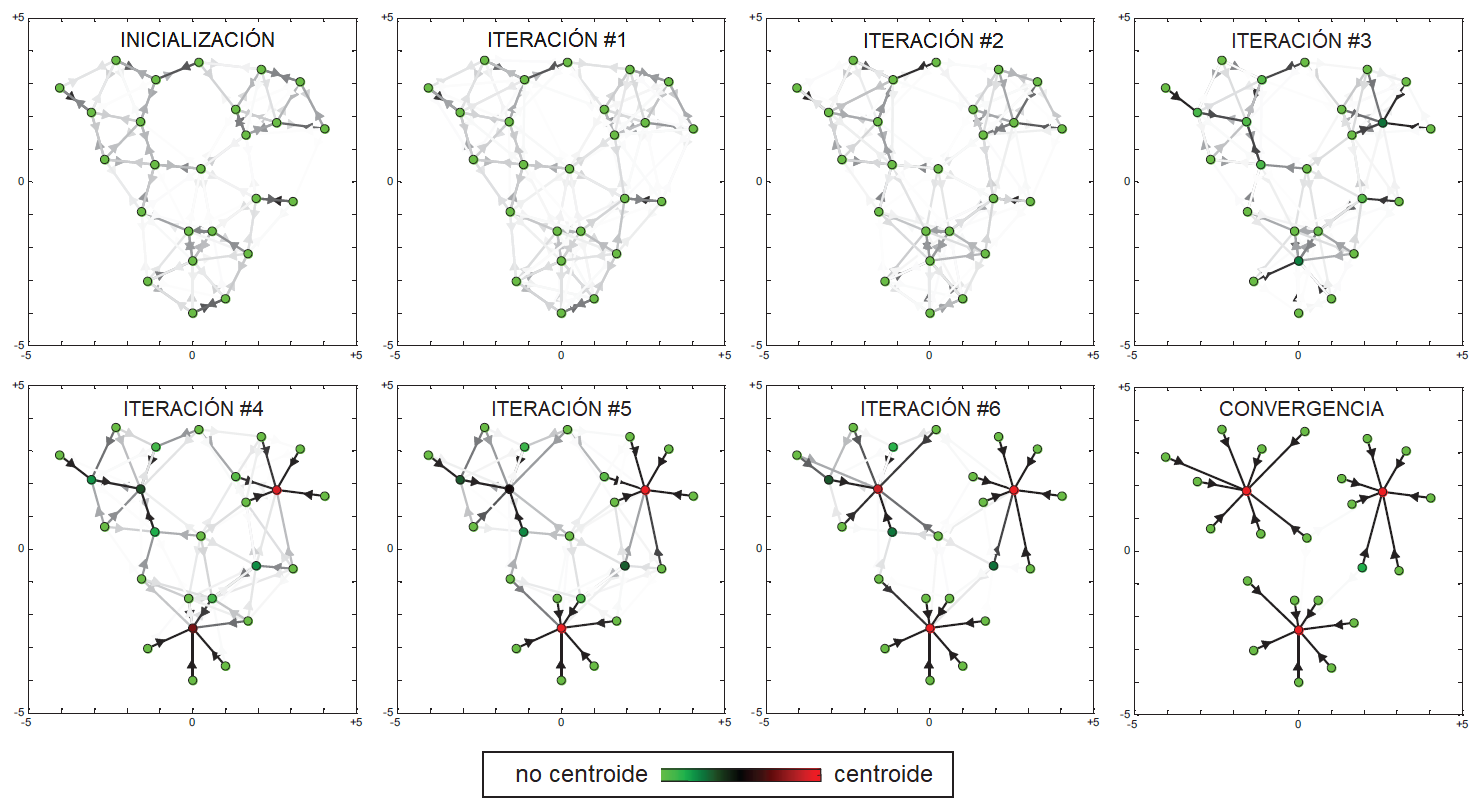
\includegraphics[width=\textwidth]{affinity-propagation.png}
    \caption{Ejemplo de ejecución del algoritmo \textit{Affinity Propagation}. El color de cada punto indica cuán cerca se encuentra de ser centroide. La tonalidad de las flechas refleja la responsabilidad entre sus extremos. (Tomado de~\cite{Murphy12})}
    \label{img:affinity-propagation}
\end{figure}

\subsubsection{Complejidad espacial y temporal}

El algoritmo Affinity Propagation tiene una complejidad temporal $O(N^2 \cdot T)$, con $N$ número de elementos del conjunto de datos y $T$ cantidad de iteraciones hasta converger, para grafos densos.
Para matrices esparcidas (correspondientes a grafos densos), el comportamiento en tiempo del algoritmo es, en cambio, $O(E\cdot T)$, con $E$ número de aristas (valores distintos de cero).

En el caso de la complejidad espacial, la memoria ocupada es $O(N^2)$ y $O(E)$ en dependencia si la matriz es esparcida o no, respectivamente~\cite{Murphy12}.


